\begin{flushleft}
\subsection{Casual use-cases}
\doublespacing


Til projektet har vi udarbejdet en liste over use-cases

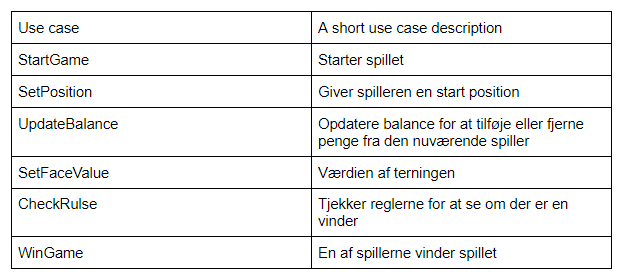
\includegraphics[width=1\textwidth]{Report/figures/Use case.PNG}
Figur 4.1.1. Tabel over casual use-cases for Monopolyspillet.
\newpage
\subsection{Fully dressed use-case}
Udover vores causal beskrevede use-cases har vi lavet en fully dressed beskrivelse til en af de mest centrale use-cases, Roll Dice.
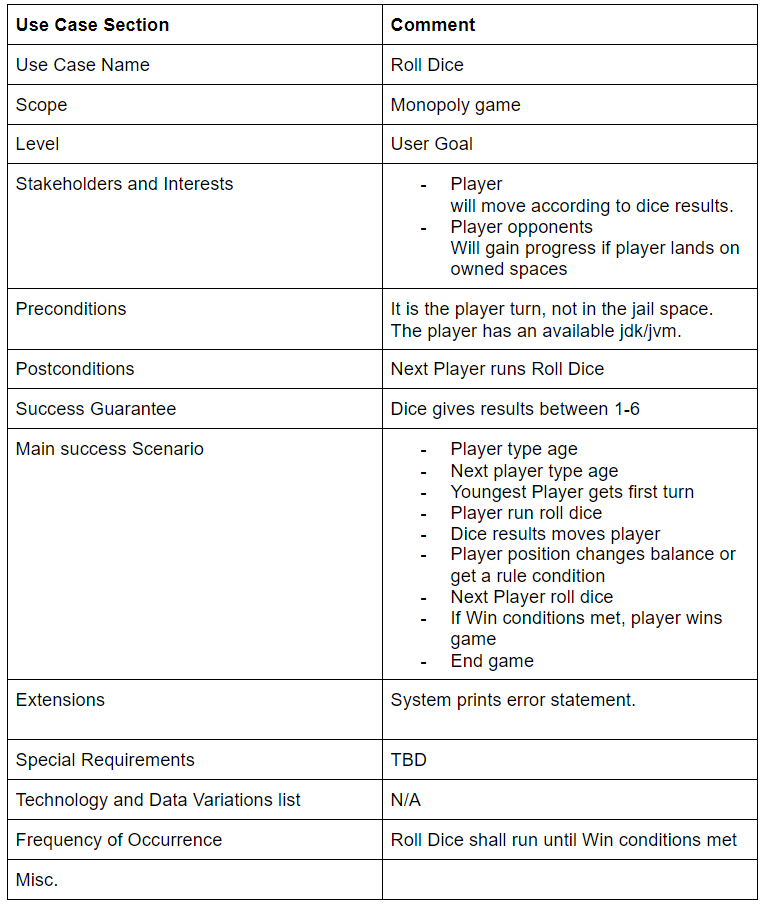
\includegraphics[width=1\textwidth, height = 18cm]{Report/figures/Fullyusecase.png}\\[0cm]
Figur 4.2.1. Tabel over fully dressed use-cases.

\subsection{Use-case diagram}
    Som en central del af analysefasen har vi udarbejdet et use-case diagram, der illustrerer de forskellige interaktioner en Player har med Monopoly spillet (se figur 4.3.1.). Det ses, at en Player kan 'Roll Dice', som herefter har en extend til 'Choose Gameboard Field' - hvilket vil sige, at Player i visse tilfælde skal kunne vælge at rykke til et felt på gameboard afhængigt af om der trækkes et specifikt Chance Card.
    \addlinespace
    Den anden centrale use-case, vi har etableret er 'Start Game'. Her kan en Player altså starte spillet, hvorefter det følger, at Player skal kunne 'Enter Name', 'Enter Player Amount' og 'Enter Age'.
    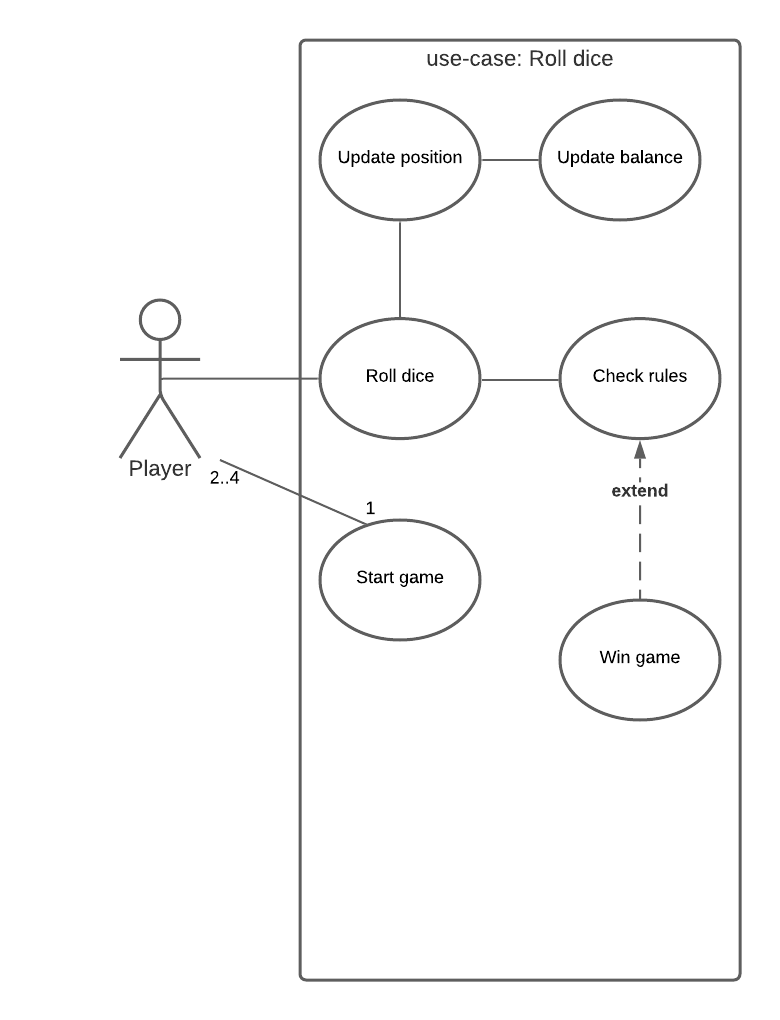
\includegraphics[width=0.9\textwidth, height = 12cm]{Report/figures/Use case diagram CDIO del3.png}~\\[0.5cm]
    Figur 4.3.1. Use-case diagram over Monopoly spillet.

\subsection{Domæne model}
    Ud fra de foregående analyser over aktører og use-cases har vi brainstormet domænet, som Monopoly spiller strækket sig over (se figur 4.4.1). Her ses det centrale objekt i domænet, som er MonopolyGame, som indeholder to til fire Player, 18 ChanceCard, én Dice og én Field. Hver Player har hver en Account, som er påvirket af Field. Yderligere har Field fire forskellige felter: JailField, ChanceField, CustomField, PropertyField og StartField, som har hhv. forskellige multipliciteter. \includegraphics[width=1\textwidth]{Report/figures/Domæne Model.png}~\\[1cm]
    Figur 4.4.1. Domæne model over Monopoly Junior spil.

\subsection{Systemsekvensdiagram}
    Som afsluttende segment i analysedelen har vi udarbejdet et systemsekvensdiagram over Monopoly Junior spillet (se figur 4.5.1). Her ses en Player og dets interaktion med Game. Først starter Player et spil via startGame, hvorefter en Player indtaster informationer vedr. antal spillere, navn og alder (enterPlayerAmount, enterPlayerName, enterPlayerAge). Herefter initieres et en løkke, Loop, der kører indtil en spiller, Player, har vundet. I løkken vises først, hvilken spillers tur det er. Herefter kan Player slå med terningen, rollDice, hvorefter der returneres værdier for terningen, den nye position, spilregler, kontobalance og næste spiller.
    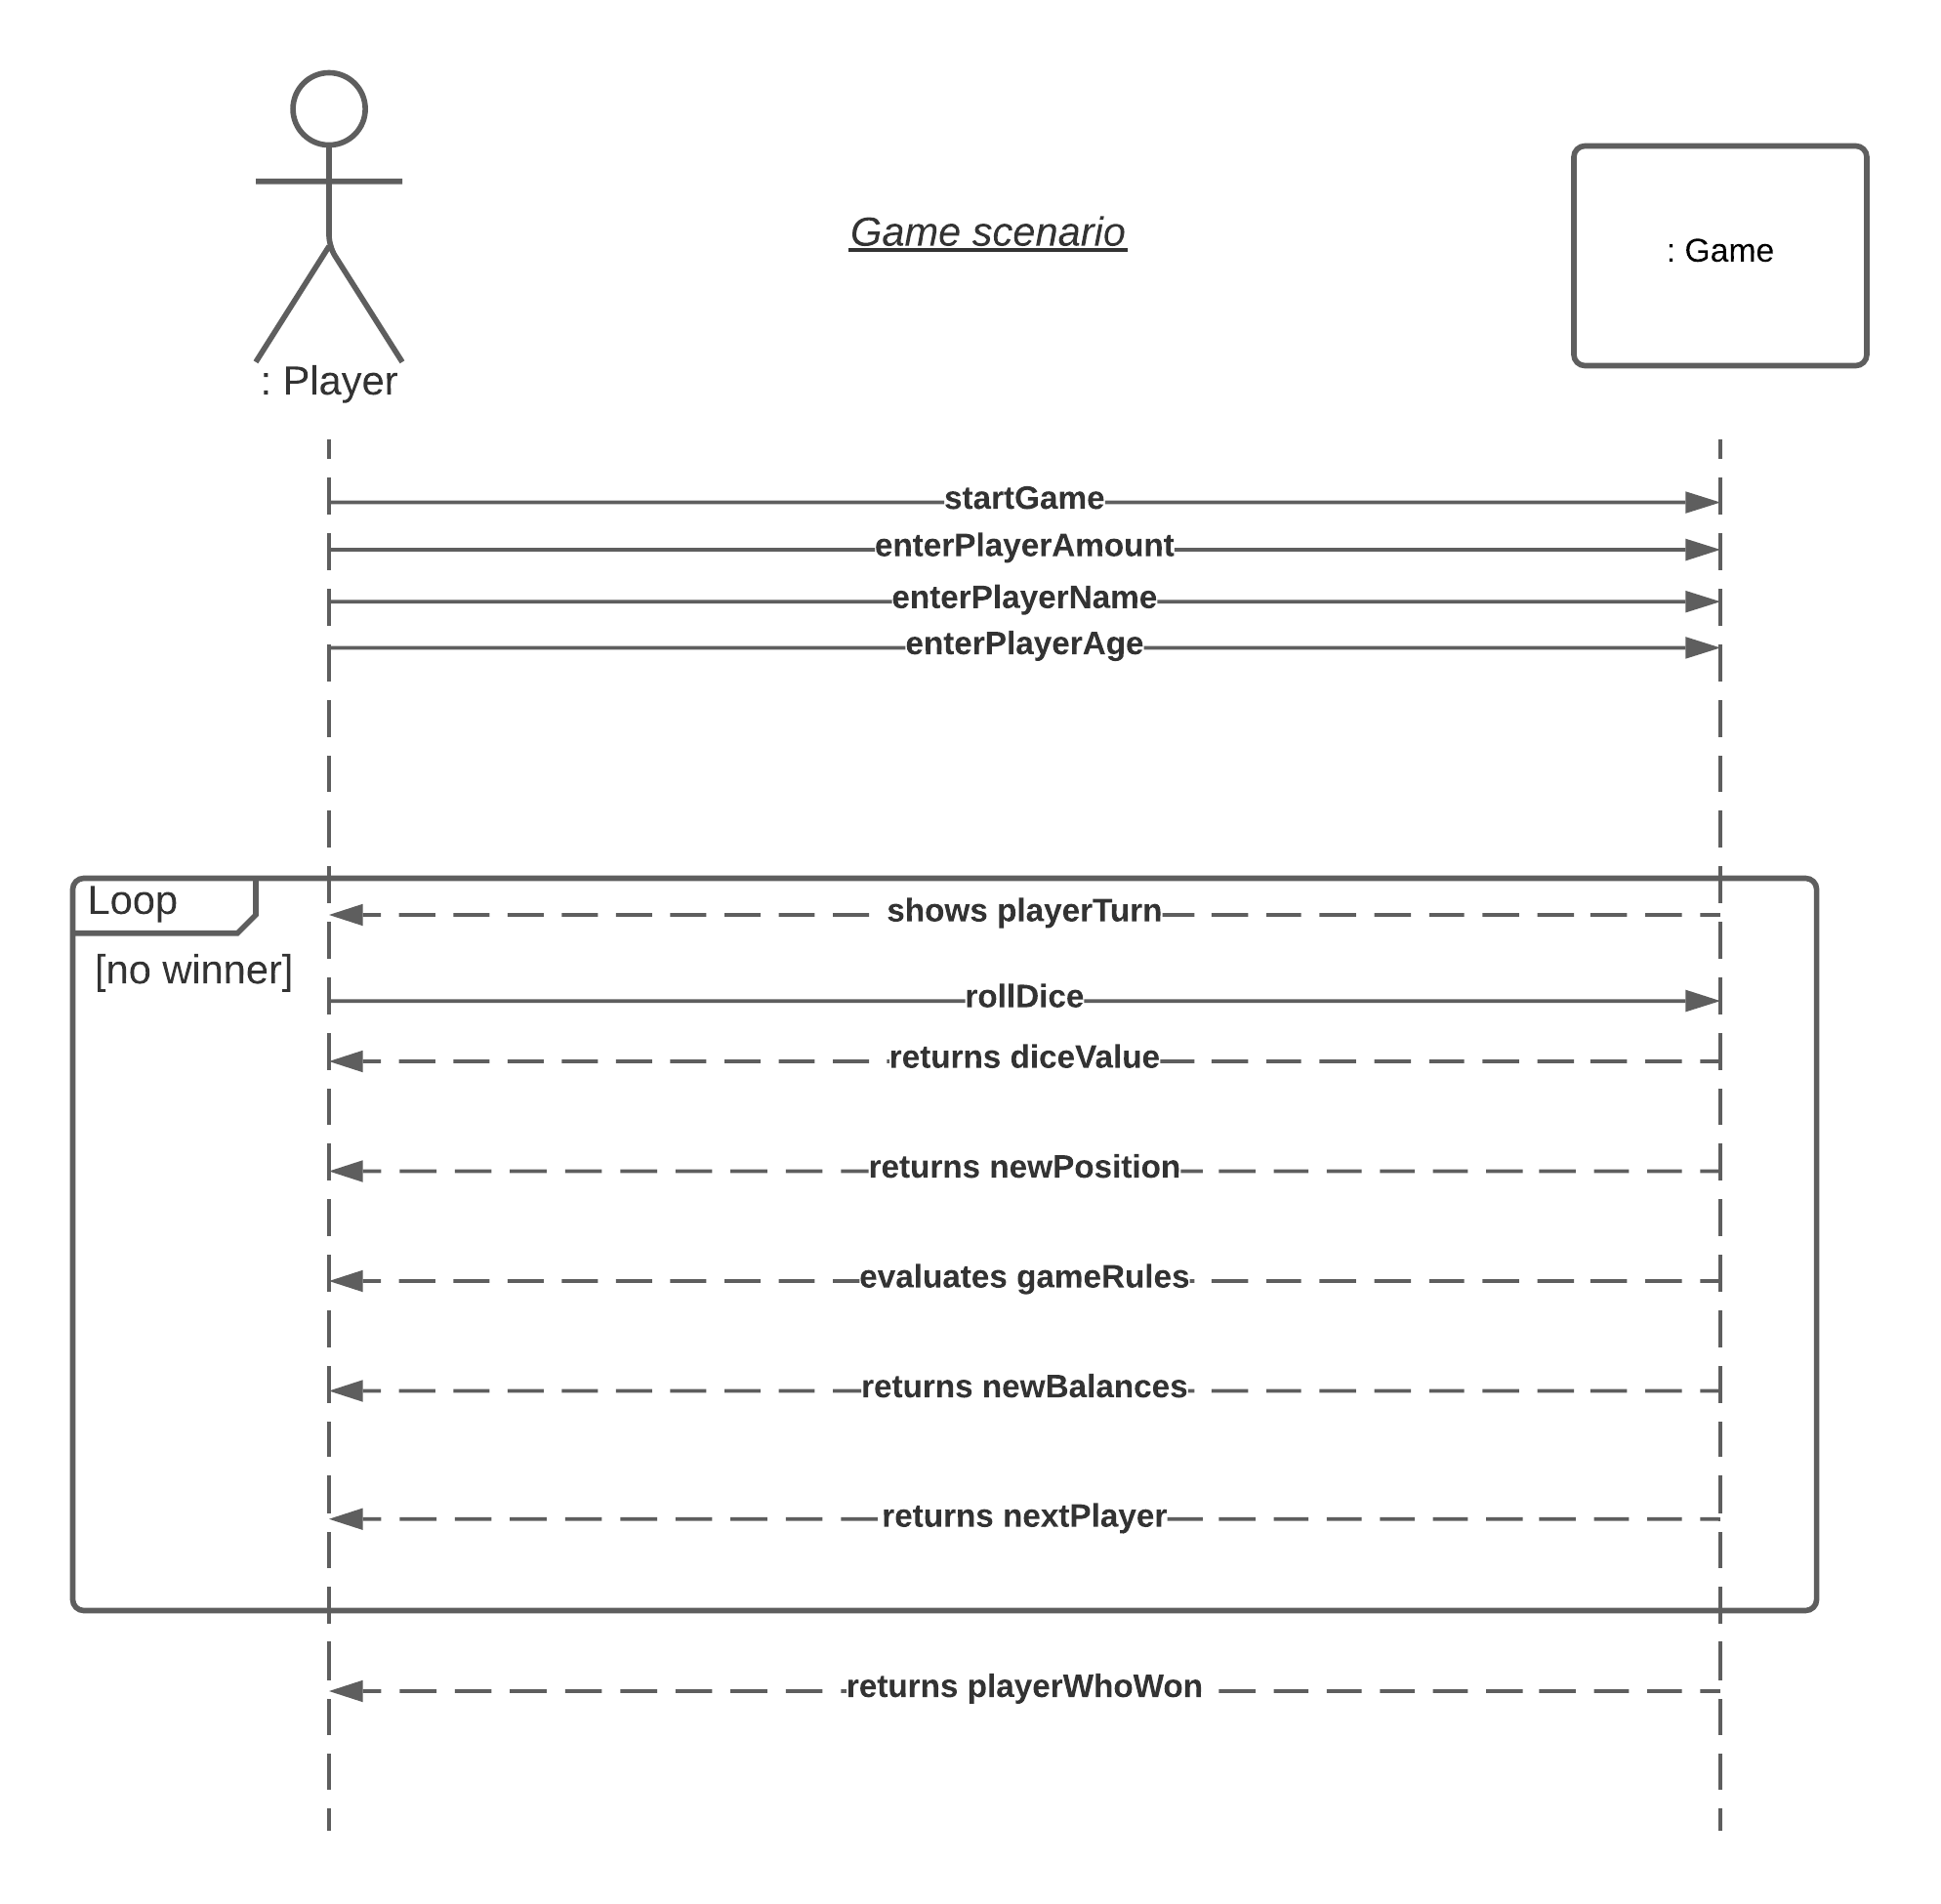
\includegraphics[width=1\textwidth, height = 13 cm]{Report/figures/System sekvensdiagram.png}~\\
    Figur 4.5.1. Systemsekvensdiagram over Monopoly Junior spillet.

\end{flushleft}